\section{Wstęp}
%Część ta~zawiera wstępne informacje o~realizowanym projekcie. Zebrano w~nim wszystko to~co było dostępne zanim student przystąpił do~realizacji informatycznej części projektu. Opisano stanowisko laboratoryjne na~którym powstał projekt.

\subsection{Geneza}
Tematem projektu, którego dotyczy ta praca jest: „Syst". Pomysł na~projekt pojawił się po~zrealizowaniu przez autora projektu semestralnego z~przedmiotu Sterowniki PLC.

\subsection{Temat}
Głównymi celami pracy było napisanie oprogramowania

\subsection{Stanowisko}
\subsubsection{Stanowisko prototypowe}
\begin{figure}[!htb] 	\centering 	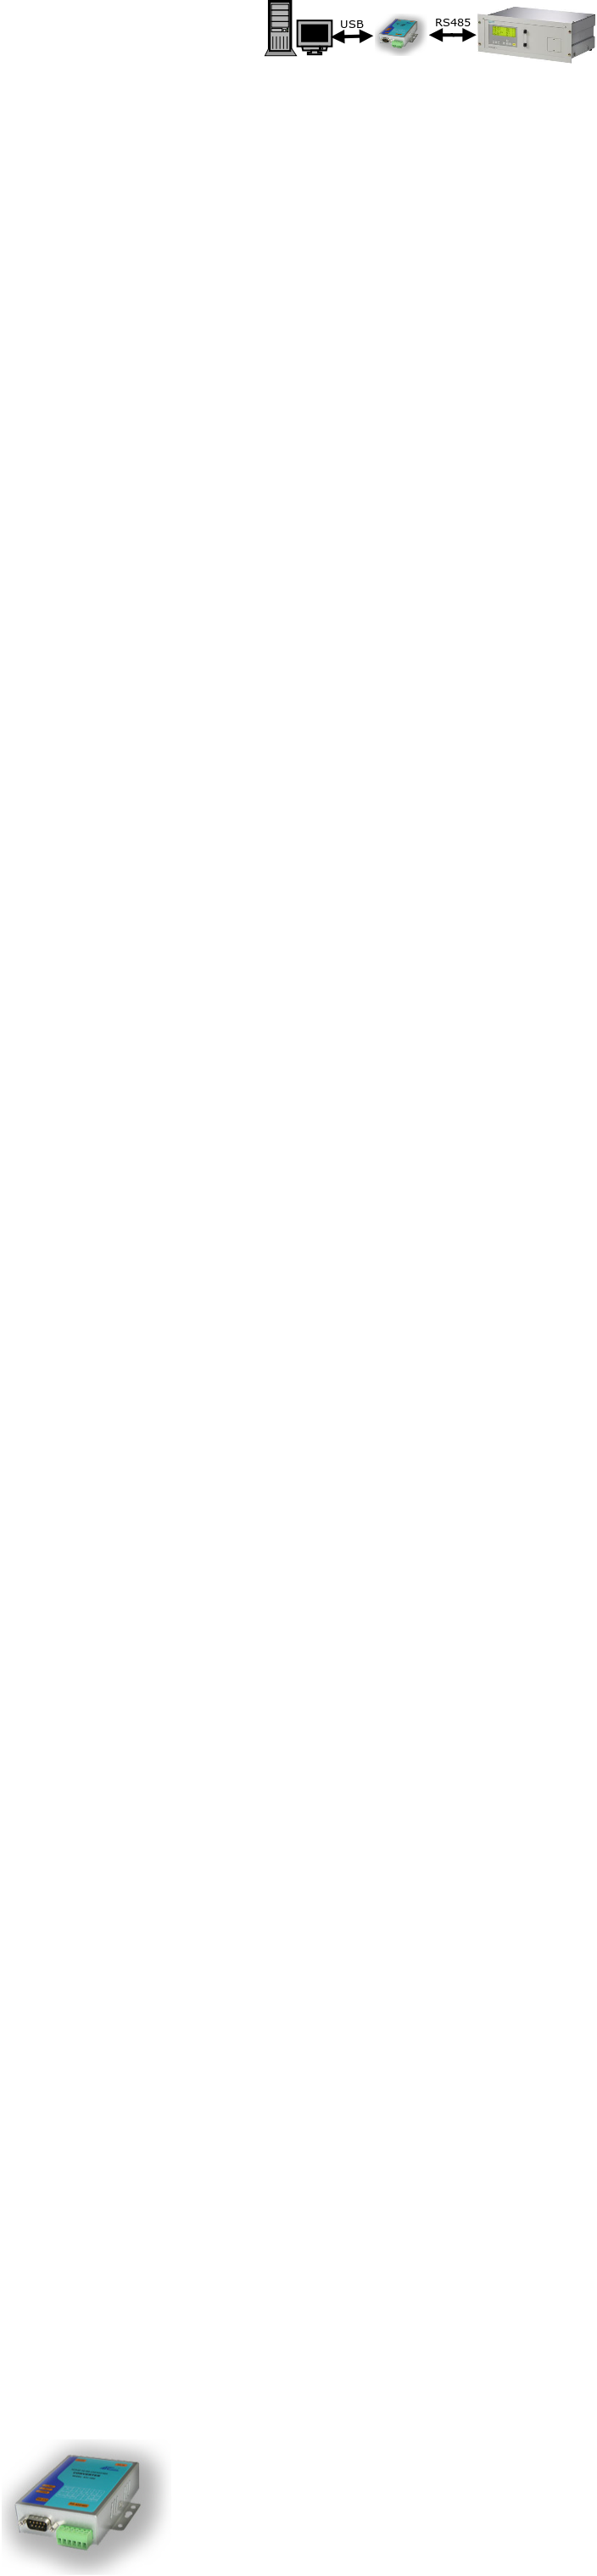
\includegraphics[width=0.8\textwidth]{images/schemat1} 	\caption{Schemat stanowiska prototypowego} \label{schemat1} \end{figure} 
Na potrzeby realizacji projektu stworzono stanowisko laboratoryjne, którego schemat przedstawia Rysunek~\ref{schemat1}. Składa się ono~z:
\begin{itemize}
\item Komputera,
\item ULTRAMAT 23
\item Konwertera ATC-850.
\end{itemize}
\indent
\indent Komputery na, których powstała wersja rozwojowa projekty pracowały na systemach operacyjnych Linux Ubuntu w wersji 32 oraz 64 bitowej. Do połączenia komputera z urządzeniem ULTRAMAT 23 zastosowano izolowany konwerter USB do RS-232/422/485, moduł ATC-850 jest automatycznie wykrywany i instalowany jako standardowy port COM. Stosowane w tej fazie projektu urządzenie pomiarowe potrafiło mierzyć zawartość $ CO_2 $, $ CO $, $ O_2 $ oraz $ NO_2 $ ??

\subsubsection{Stanowisko docelowe}
\begin{figure}[!htb] 	\centering 	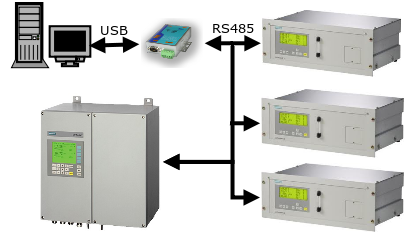
\includegraphics[width=0.8\textwidth]{images/schemat2} 	\caption{Schemat stanowiska docelowego} \label{schemat2} \end{figure} 
Docelowo zrealizowany projekt ma być uruchamiany na stanowisku, którego schemat przedstawia Rysunek~\ref{schemat2}. Składa się ono~z:
\begin{itemize}
\item Komputera,
\item 3x ULTRAMAT 23
\item ULTRAMAT 6
\item Konwertera ATC-850.
\end{itemize}
\indent
\indent aaaa
\end{enumerate}

\subsection{Analiza tematu}
Analiza tematu polegała przede wszystkim na zapoznaniu się z~narzędziami programistycznymi do~tworzenia oprogramowania sterownika oraz wizualizacji.
W~wyniku analizy autor poznał podstawy języków: LAD~\cite{step1,step2,step3}, STL~\cite{step1,step2,step3}, FBD~\cite{step1,step2,step3}, GRAPH~\cite{step3}, SCL~\cite{scl1,scl2,scl3} i AWL do~tworzenia programu sterownika oraz VBScript do~tworzenia skryptów w~wizualizacji. Poznanie tych podstaw pozwoliło dobrać język odpowiedni do~realizacji poszczególnych zadań.

\subsection{Założenia}
%Stworzone oprogramowanie dla Robota Fishertechnik ma działać na sterownikach firmy Siemens oraz ma zostać stworzone przy użyciu środowiska Step 7. Funkcjonalności robota, jakie mają wchodzić w~skład projektu, to:
Oprogramowanie dla Robota Fishertechnik powinno zostać stworzone przy użyciu środowiska Step 7 oraz działać na sterownikach firmy Siemens. Funkcjonalności robota wchodzące w~skład projektu, to:
\begin{itemize}
\item sterowanie ręczne z~pilota podłączonego bezpośrednio do~sterownika,
\item sterowanie ręczne z~wizualizacji,
\item sterowanie automatyczne, 
\item wizualizacja stanu magazynu,
\item umożliwienie korzystania z~magazynu zarówno poprzez sterowanie ręczne, jak i~przy użyciu zautomatyzowanych poleceń dostępnych z~poziomu wizualizacji.
\end{itemize}
\indent
\indent Powyżej zostały wymienione założenia podstawowe, jednak autor nie wyklucza zrealizowania dodatkowych zadań, które nie zostały zamieszczone w~pierwotnej koncepcji realizacji projektu.
%Zamieszczone tu założenia są podstawowe, ale niewykluczone jest zrealizowanie przez autora dodatkowych zadań nie zaplanowanych przed rozpoczęciem realizacji projektu.

\subsection{Plan pracy}
Realizacja projektu została podzielona na następujące etapy:
\begin{itemize}
\item Przygotowanie stanowiska, zebranie odpowiednich materiałów i~literatury,
\item Analiza wymagań funkcjonalnych aplikacji,
\item Projektowanie struktury oprogramowania i~interfejsów wymiany danych,
\item Implementacja,
\item Testowanie i~uruchamianie,
\item Przedstawienie projektu i~ewentualne korekty.
\end{itemize}
\indent
\indent Powyższy plan pracy stanowił dla autora wyznacznik kolejnych działań. Jednak powszechnie wiadomo, że w~praktyce poszczególne punkty są~wymienne i~wpływają na siebie wzajemnie.
